\documentclass{article}
\usepackage{tikz}
\author{Asher Griess, David Medin}
\title{R Tree Algorithm}
\begin{document}
\maketitle

\section{Abstract}
An R Tree is a data structure used to make spacial computation and comparison much faster than brute force.  ...

\section{Use Cases}
The R-tree is very similar to the B-tree in structure, and Quad-Tree in use. One of the main differences is that
R-trees are page-able. This means that they could be put into storage, which could be ideal for very large data sets
that can't be stored in ram. You can also take out parts of the R-tree into ram while working with it. A good example
of a program that could use R-trees is a mapping system of the world, where the large data set would be hard to store in memory.
The R-tree is also very good for nearest neighbor searching. Also R-tree can be used to store any type of shape which allow for shapes
of things such as buildings to be put in the minimum bounding rectangle. R-trees have also been used a lot in databases for spacial data.


\section{Inserting}
Complexity

average : none

worst case : $O(n)$

When splitting we are trying to find the best leaf node
that will have least increase to the minimum bounding rectangle.
It should also be noted that when we are at M leafs at every node we are going
to need to perform a split where M is the max children per node.

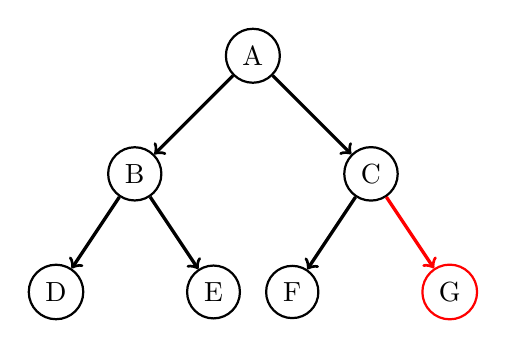
\begin{tikzpicture}
\begin{scope}[every node/.style={circle,thick,draw}]
    \node (A) at (2.5,4) {A};
    \node (B) at (1,2.5) {B};
    \node (C) at (4,2.5) {C};
    \node (D) at (0,1) {D};
    \node (E) at (2,1) {E};
    \node (F) at (3,1) {F} ;
    
\end{scope}

\begin{scope}[every node/.style={circle,thick,draw=red}, 
    every edge/.style={draw=red,very thick}]
    \node (G) at (5,1) {G};
    \path [->] (C) edge (G);
    
\end{scope}

\begin{scope}[every edge/.style={draw=black,very thick}]
              \path [->] (A) edge (B);
              \path [->] (A) edge (C);
              \path [->] (B) edge (D);
              \path [->] (B) edge (E);
              \path [->] (C) edge (F);
\end{scope}
\end{tikzpicture}

In this figure we would be adding the node G as a child of G
if C's minimum boudning box increases the least.
\subsection*{Psuedo Code}
\begin{flushleft}
    
If at leaf:

\quad Insert Entry

\quad If entries $>$ M

\quad \quad Split

\quad Return

If Entry fits in to any of the children.

 \quad Recurse into node


else:

\quad For each child:

    \quad \quad
    Find difference in area if Entry were inserted

    \quad Recurse into to node with smallest difference
\end{flushleft}

\section{Splitting} 

\section{Searching}
Complexity
Average : $O(log_Mn)$
Worst Case : $O(n)$

\section{Removing}
\paragraph{}
When removing a point - or an object - from a R Tree, the first step is to find the leaf node that stores the point.
However, we have already covered that in the previous section, Searching. Now that we have the leaf node that contains
the point, we now remove the point from the leaf node. This may reduce the number of entries this leaf node has to be below
$M/2$, which is not allowed for nodes that are not root. If the leaf node is the root then we ignore this problem, because
we can't have a smaller tree.
\paragraph{}
If this node is not the root and has less than $M/2$ entries, then it is necessary to delete that node. But we don't want to destroy
the other $M/2 - 1$ nodes, so we'll store each of the node's entries into a list, or other container type, to insert back into
the tree when we are done removing. Because we are removing the leaf node, this means that its parent's entries can also fall below
$M/2$ nodes, which then requires that it is deleted too. In that case, a recursive search of all of that parent's children is necessary
to find all points - or other data objects - to store for reinsertion later.
\paragraph{}
Even though it seems that a the leaf node case and the parent node case seem different, they are actually the same case. Parents have
other nodes as their entries and leaf nodes have objects as their entries. Both must have $M/2 \le n \le M$ entries (where $n$ is the number
of entries the node has), and both need to be deleted from their parent and recursively store all of the entries below it in the tree.

\section{Citation}

% text \textbf{bold text} text. Some math: $2+2=5$

% \begin{tikzpicture}[main/.style = {draw, circle}]
% \node[main](1){$x_1$};
% \end{tikzpicture}

\end{document}